Reazioni in cui mettiamo a reagire un acido e una base.
\subsection{Esempi}
\ce{HCl(aq) + NH_3(aq) <--> NH_4^+(aq) + Cl^-(aq)}

\vspace{0.2cm}(Nota: sia accanto all'acido cloridrico che all'ammoniaca c'è scritto acquoso (aq), perché entrambe le specie sono gas. Noi li facciamo gorgogliare in acqua, ottenendo delle soluzioni acquose dell'acido e della base. Stiamo quindi immaginando di avere due soluzioni acquose che mescoleremo insieme)

Questa reazione produce lo ione $\rm NH_4^+$, in quanto l'acido cloridico è un acido forte, totalmente dissociato, quindi con $\rm HCl(aq)$ intendiamo ione $\rm H^+$ e ione $\rm Cl^-$; non è così invece per l'ammoniaca che è una base debole. Lo ione $\rm H^+$ dell'HCl, già dissociato, protona l'ammoniaca grazie al doppietto presente sull'azoto dell'$\rm NH_3$ (infatti tale doppietto è adatto a legare questo ulteriore protone), formando lo ione $\rm NH_4^+$, mentre dall'HCl resta lo ione cloruro $\rm Cl^-$.

Questa è una reazione acido-base, per cui si forma un sale che è il cloruro di ammonio, il quale in acqua, come tutti gli elettroliti forti, è totalmente dissociato, infatti nella reazione c'è una singola freccia. Va poi da ricordare che tutti i sali sono elettroliti forti per definizione.

\vspace{0.2cm}\ce{CH_3COOH + H_2O(l) <--> CH_3COO^- + H_3O^+(aq)}

\vspace{0.2cm}L'acido acetico in acqua si dissocia, liberando un protone che si somma all'acqua usando il doppietto dell'ossigeno disponibile per legarlo, formando lo ione $\rm H_3O^+$. Dell'acido resterà lo ione acetato $\rm CH_3COO^-$.

Questa reazione non è tutta spostata verso destra, per cui mettiamo le doppie frecce. Infatti questa seconda reazione è la dissociazione di un acido debole.

\vspace{0.2cm}\ce{CH_3COOH + HClO_4(aq) <--> CH_3COOH_2^+(aq) + ClO_4^-(aq)}

\vspace{0.2cm}In questa terza reazione abbiamo due acidi: acido acetico e acido perclorico. Abbiamo visto che ci sono speci anfotere, cioè che si comportano o da acido o da base a seconda del partner. Da un punto di vista formale allora, possiamo "forzare la mano" e scegliere una specie etichettata acida per dimostrare che anch'essa può comportarsi da base se in presenza di un acido estremamente più forte: sebbene l'acido acetico sia un acido, se è in soluzione con un acido molto più forte (l'acido perclorico è l'acido più forte che esista) anziché dissociarsi cedendo un protone e rimanendo ione acetato vedrà l'$\rm HClO_4$ cedere un protone, formando lo ione $\rm ClO_4^-$. Questo protone si somma all'acido acetico ottenendo la specie $\rm CH_3COOH_2^+$, ione acidioacetato. Quindi in questa reazione, avendo forzato molto, l'acido acetico si è comportato da base, perché ha accettato il protone.

Attenzione! Ciò non implica che l'acido acetico sia un afolita. Questo esempio serve solo 

\begin{center}
    \begin{tabular}{llllllll}
        \textbf{Nome} & \textbf{Acido 1} & & \textbf{Base 2} & & \textbf{Base 1} & & \textbf{Acido 2}\\[0.3ex]
        Acido cloridico & HCl & + & $\rm H_2O$ & \ce{<-->} & $\rm Cl^-$ & + & $\rm H_3O^+$\\[0.3ex]
        Acido nitrico & $\rm HNO_3$ & + & $\rm H_2O$ & \ce{<-->} & $\rm NO_3^-$ & + & $\rm H_3O^+$\\[0.3ex]
        Acido carbonico & $\rm H_2CO_3$ & + & $\rm H_2O$ & \ce{<-->} & $\rm HCO_3^-$ & + & $\rm H_3O^+$\\[0.3ex]
        Acido acetico & $\rm CH_3CO_2H$ & + & $\rm H_2O$ & \ce{<-->} & $\rm CH_3CO_2^-$ & + & $\rm H_3O^+$\\[0.3ex]
        Acido cianidrico & $\rm HCN$ & + & $\rm H_2O$ & \ce{<-->} & $\rm CN^-$ & + & $\rm H_3O^+$\\[0.3ex]
        Acido solfidrico & $\rm H_2S$ & + & $\rm H_2O$ & \ce{<-->} & $\rm HS^-$ & + & $\rm H_3O^+$\\[0.3ex]
        Ammoniaca & $\rm H_2O$ & + & $\rm NH_3$ & \ce{<-->} & $\rm OH^-$ & + & $\rm NH_4^+$\\[0.3ex]
        Ione carbonato & $\rm H_2O$ & + & $\rm CO_3^{2-}$ & \ce{<-->} & $\rm OH^-$ & + & $\rm HCO_3^-$\\[0.3ex]
        Acqua & $\rm H_2O$ & + & $\rm H_2O$ & \ce{<-->} & $\rm OH^-$ & + & $\rm H_3O^+$\\[0.3ex]
    \end{tabular}
\end{center}

Nelle reazioni ci devono essere almeno due partner, perché non esiste un acido se non c'è una base, cioè se una specie cede protoni è indispensabile che ci sia un'altra specie che li acquisti, quindi sia a sinistra che a destra della reazione devono esserci almeno due composti.

Nelle prime sei reazioni l'acqua si comporta da base, acquistando un protone e diventando ione $\rm H_3O^+$, specie che a sua volta potrà cedere un protone, quindi è un acido. Chiaramente lo ione che resta dalla dissociazione dell'acido sarà la base coniugata.

Nelle due successive l'acqua è in presenza di basi, per cui si comporta da acido, dunque sarà la specie che cede il protone, dando lo ione $\rm OH^-$ in soluzione che è la base coniugata.

Nell'ultima reazione vediamo che due molecole d'acqua danno luogo ad uno ione $\rm H_3O^+$ e ad uno ione $\rm OH^-$. Approfondiremo.
\subsection{Sistemi acido-base secondo Brönsted}
Per generalizzare il comportamento che abbiamo descritto non possiamo parlare di acido o di base, ma di sistemi acido-base.

Dato che gli acidi cedono protoni, li etichettiamo con H-A e con $\rm H^+$ indichiamo il protone e con $\rm A^-$ ciò che resta. Etichettiamo invece con B la base, che sarà tale se e solo potrà acquistare il protone:

\begin{figure}[H]
    \centering
    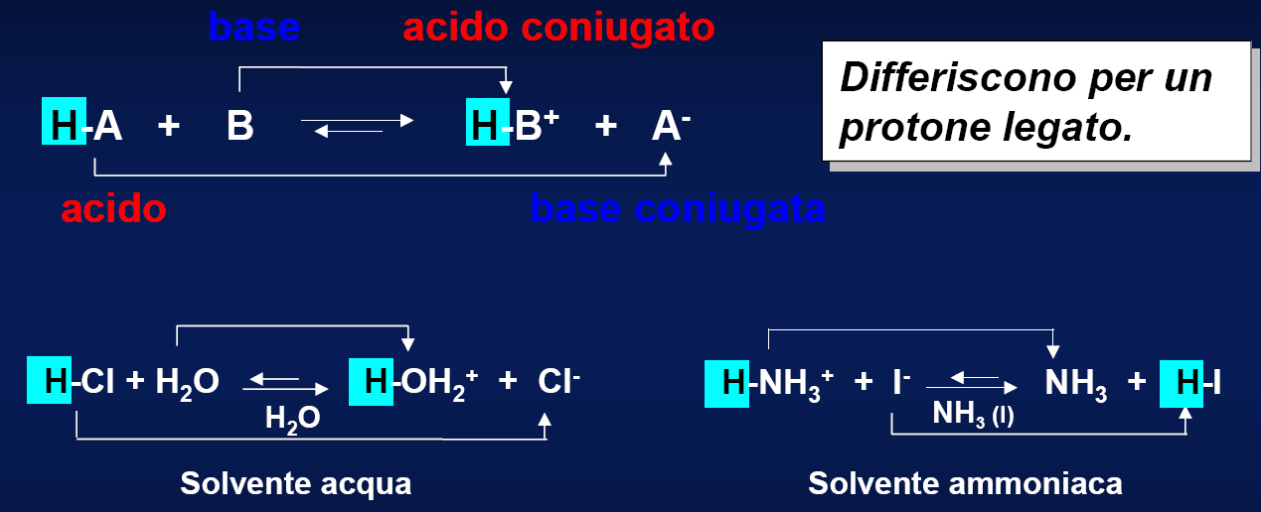
\includegraphics[width=14cm]{immagini/acido_base_coniugata.png}
\end{figure}

\subsection{Forza degli acidi e delle basi}
\textbf{ES.}

$$\ce{HCOOH(aq) + H_2O(l) <--> HCOO^-(aq) + H_3O^+(aq)}$$

L'acido formico in acqua dà lo ione formiato, e il protone che si libera si associa all'acqua per formare $\rm H_3O^+$.

$$k= \rm{\frac{[HCOO^-]\cdot[H_3O^+]}{[HCOOH]}} = \frac{\alpha^2}{1- \alpha}\textit{c}$$
\subsection{Autodissociazione dell'acqua}
Abbiamo visto la reazione

$$\ce{H_2O + H_2O <--> H_3O^+ + OH^-}$$

In essa stiamo immaginando di avere soltanto acqua a disposizione. Ciononostante l'acqua si autodissocia producendo, tramite un equilibrio, un po' di ioni $\rm H_3O^+$ e un po' di ioni $\rm OH^-$.

Se così fosse l'acqua pura dovrebbe condurre. Con una misura di conducibilità possiamo risalire alla concentrazione di questi ioni. Vedremo che essa è molto piccola, per cui l'autodissociazione dell'acqua sarà trascurabile.

La costante è data da

$$\ce{2 H_2O <--> H_3O^+ + OH^-}
\implies
k= \frac{[\text{H}_3\text{O}^+] [\text{OH}^-]}{[\text{H}_2\text{O}]^2} \; (=1.8 \cdot 10^{-16})$$

$$\implies k \cdot [\text{H}_2\text{O}]^2 = [\text{H}_3\text{O}^+] \cdot [\text{OH}^-] = k_w$$

Poniamo $k_w$ il prodotto di $k$ per la concentrazione dell'acqua all'equilibrio al quadrato, che si vede essere pari anche al prodotto della concentrazione dello ione $\rm H_3O^+$ per quella dello ione $\rm OH^-$. Inoltre quest'ultime due concentrazioni saranno uguali, perché ogni due molecole di acqua si producono uno ione $\rm H_3O^+$ e uno ione $\rm OH^-$. Si trova infatti che entrambe sono pari a $10^{-7}$ mol/L.

Va da notare che se le quantità degli ioni sono uguali, non ci sarà un eccesso di $\rm H_3O^+$ che porta l'acqua ad essere acida né un eccesso di ioni $\rm OH^-$ che porta l'acqua ad essere basica: l'acqua è neutra, poiché questi ioni hanno stessa concentrazione.

$$k_w = 10^{-7} \, (mol/L) \cdot 10^{-7} \, (mol/L) = 10^{-14}$$
\subsection{Il pH}
$$\log \left( \frac{1}{k_w} \right) = \log \left( \frac{1}{\rm{[H_3O^+]}} \right) + \log \left( \frac{1}{\rm{[OH^-]}} \right) = \log \frac{1}{10^{-14}}=14$$

$$\text{p}k = \log \frac{1}{k}; \quad \rm pH = \log \frac{1}{[H_3O^+]}; \quad pOH = \log \frac{1}{[OH^-]}; \quad$$

$$\implies \rm pH + pOH = 1$$

\subsubsection{Definizioni: pH e P$\boldsymbol{k_a}$}

\subsubsection{Definizioni: pOH e P$\boldsymbol{k_w}$}

\subsubsection{Definizioni: P$\boldsymbol{k_a}$ vs P$\boldsymbol{k_b}$}

\ce{HA <--> H^+ + A^-}

In questa reazione abbiamo un acido che si dissocia in $\rm H^+$ + $\rm A^-$. Correttamente dovremmo scrivere

$$\ce{HA + H_2O <--> H_3O^+ + A^-}$$

Per questa prima specie calcoliamo $k_a$, data da

$$k_a = \left( \rm \frac{[H^+] \cdot [A^-]}{[HA]} \right)$$

Se ad esempio HA fosse l'acido acetico, e anziché metterlo in acqua prendessimo un suo sale come l'acetato di sodio, quest'ultimo, come tutti i sali, si dissocerà totalmente in ioni acetato e ione $\rm Na^+$. Lo ione acetato è la base coniugata dell'acido acetico, in quanto è ottenuto a partire da questo togliendo un protone.

Che succede alla base coniugata di un qualunque acido??

Va da ricordare che se l'acido è debole, la sua base coinugata è forte. Ne segue che la $k_b$ è grande.

\vspace{0.2cm}\ce{A^- + H_2O <--> HA + OH^-}

\vspace{0.2cm}Se mettiamo lo ione $\rm A^-$ (ione acetato nel nostro esempio), questo strappa un protone all'acqua perché è una base forte, formando la specie HA che in teoria è un acido, ma se non si dissocia non manifesta le proprietà acide.

Avendo tolto un protone ad $\rm H_2O$, ci sarà rimasto un eccesso di $\rm OH^-$. Abbiamo quindi scoperto che avevamo messo in acqua un sale neutro e la reazione è basica. Questo perché le basi coniugate degli acidi deboli sono basi forti.

Ciò che succede è che quando mettiamo un sale neutro in acqua questo si dissocia, l'anione poi strappa un protone all'acqua e libera ioni $\rm OH^-$, ottenendo così una soluzione basica.

Ci sarà allora una costante basica, pari a

$$k_b = \left( \rm \frac{[OH^-] \cdot [HA]}{[A^-]} \right)$$

Consideriamo ora il prodotto di $k_a$ e $k_b$

$$k_a \cdot k_b = \left( \rm \frac{[H^+] \cdot [A^-]}{[HA]} \right) \cdot \left( \rm \frac{[OH^-] \cdot [HA]}{[A^-]} \right)$$

$$\implies k_a \cdot k_b = \rm [H^+] \cdot [OH^-] \equiv \textit{k}_\textit{w}$$

Ecco perché se una cresce l'altra diminuisce: perché il loro prodotto deve essere pari a $10^{-14}$ sempre.

Quindi il prodotto della costante di un acido e della costante della sua base coniugata darà sempre il prodotto ionico dell'acqua $k_w$, per cui si avrà sempre che se l'acido è debole la base coniugata sarà forte, mentre se l'acido è forte la sua base coniugata sarà debole.

\vspace{0.2cm}Esempi:
\begin{itemize}
    \item L'aicdo fluoridrico ha costante $k_a=7.2 \cdot 10^{-4}$. La sua base coniugata, lo ione fluoruro $\rm F^-$;
    \item Acido nitroso
    \item Acido solforoso
\end{itemize}